\documentclass{standalone}
\usepackage{tikz}
\usetikzlibrary{patterns, positioning}


\begin{document}
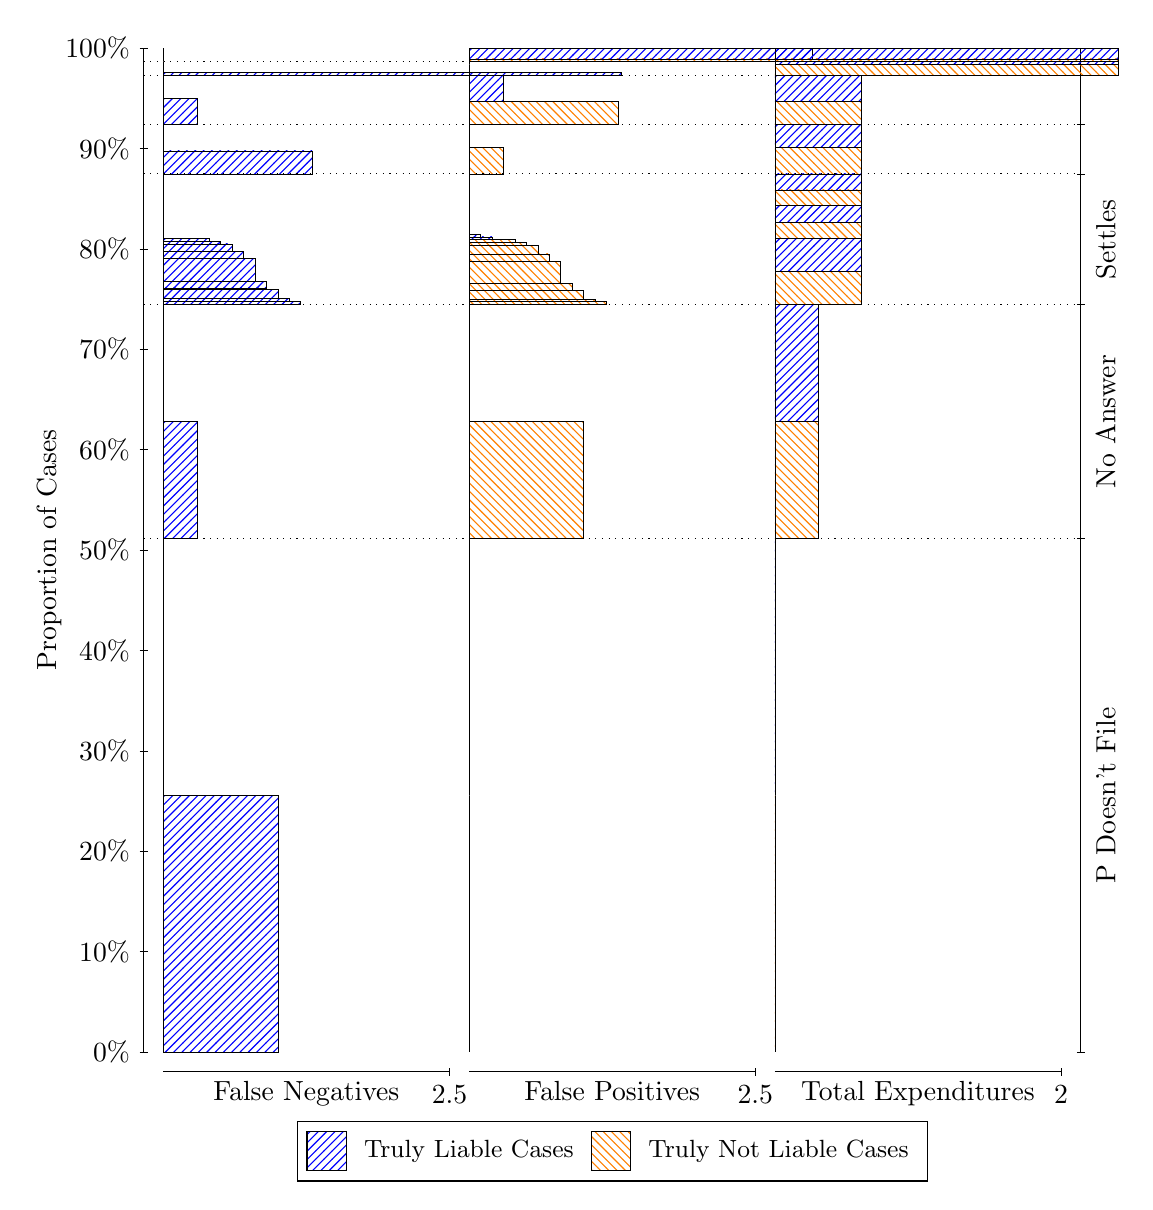
\begin{tikzpicture}
\draw[black, very thin] (1.5,1.75) -- (1.5,14.5);
\node[rotate=90, text=black, anchor=center] at (0.3, 8.125) {Proportion of Cases};
\draw[black, very thin] (1.45,1.75) -- (1.55,1.75);
\node[text=black, anchor=east] at (1.45, 1.75) {0\%};
\draw[black, very thin] (1.45,3.025) -- (1.55,3.025);
\node[text=black, anchor=east] at (1.45, 3.025) {10\%};
\draw[black, very thin] (1.45,4.3) -- (1.55,4.3);
\node[text=black, anchor=east] at (1.45, 4.3) {20\%};
\draw[black, very thin] (1.45,5.575) -- (1.55,5.575);
\node[text=black, anchor=east] at (1.45, 5.575) {30\%};
\draw[black, very thin] (1.45,6.85) -- (1.55,6.85);
\node[text=black, anchor=east] at (1.45, 6.85) {40\%};
\draw[black, very thin] (1.45,8.125) -- (1.55,8.125);
\node[text=black, anchor=east] at (1.45, 8.125) {50\%};
\draw[black, very thin] (1.45,9.4) -- (1.55,9.4);
\node[text=black, anchor=east] at (1.45, 9.4) {60\%};
\draw[black, very thin] (1.45,10.675) -- (1.55,10.675);
\node[text=black, anchor=east] at (1.45, 10.675) {70\%};
\draw[black, very thin] (1.45,11.95) -- (1.55,11.95);
\node[text=black, anchor=east] at (1.45, 11.95) {80\%};
\draw[black, very thin] (1.45,13.225) -- (1.55,13.225);
\node[text=black, anchor=east] at (1.45, 13.225) {90\%};
\draw[black, very thin] (1.45,14.5) -- (1.55,14.5);
\node[text=black, anchor=east] at (1.45, 14.5) {100\%};

\draw[black, very thin] (13.4,1.75) -- (13.4,14.5);
\draw[black, very thin] (13.35,1.75) -- (13.45,1.75);
\node[anchor=west] at (13.35, 1.75) {};
\draw[black, very thin] (13.35,8.2686) -- (13.45,8.2686);
\node[anchor=west] at (13.35, 8.2686) {};
\draw[black, very thin] (13.35,11.243) -- (13.45,11.243);
\node[anchor=west] at (13.35, 11.243) {};
\draw[black, very thin] (13.35,12.901) -- (13.45,12.901);
\node[anchor=west] at (13.35, 12.901) {};
\draw[black, very thin] (13.35,13.532) -- (13.45,13.532);
\node[anchor=west] at (13.35, 13.532) {};
\draw[black, very thin] (13.35,14.152) -- (13.45,14.152);
\node[anchor=west] at (13.35, 14.152) {};
\draw[black, very thin] (13.35,14.327) -- (13.45,14.327);
\node[anchor=west] at (13.35, 14.327) {};
\draw[black, very thin] (13.35,14.5) -- (13.45,14.5);
\node[anchor=west] at (13.35, 14.5) {};

\draw[black, very thin, pattern color=blue, pattern=north east lines] (1.75,1.75) rectangle (3.2033,5.0093);
\draw[black, very thin, pattern color=orange, pattern=north west lines] (1.75,5.0093) rectangle (1.75,8.2686);
\draw[black, very thin, pattern color=blue, pattern=north east lines] (1.75,8.2686) rectangle (2.186,9.756);
\draw[black, very thin, pattern color=orange, pattern=north west lines] (1.75,9.756) rectangle (1.75,11.243);
\draw[black, very thin, pattern color=blue, pattern=north east lines] (1.75,11.243) rectangle (3.494,11.281);
\draw[black, very thin, pattern color=blue, pattern=north east lines] (1.75,11.281) rectangle (3.3487,11.316);
\draw[black, very thin, pattern color=blue, pattern=north east lines] (1.75,11.316) rectangle (3.2033,11.435);
\draw[black, very thin, pattern color=blue, pattern=north east lines] (1.75,11.435) rectangle (3.058,11.455);
\draw[black, very thin, pattern color=blue, pattern=north east lines] (1.75,11.455) rectangle (3.058,11.539);
\draw[black, very thin, pattern color=blue, pattern=north east lines] (1.75,11.539) rectangle (2.9127,11.833);
\draw[black, very thin, pattern color=blue, pattern=north east lines] (1.75,11.833) rectangle (2.7673,11.917);
\draw[black, very thin, pattern color=blue, pattern=north east lines] (1.75,11.917) rectangle (2.622,12.012);
\draw[black, very thin, pattern color=blue, pattern=north east lines] (1.75,12.012) rectangle (2.4767,12.043);
\draw[black, very thin, pattern color=blue, pattern=north east lines] (1.75,12.043) rectangle (2.3313,12.078);
\draw[black, very thin, pattern color=orange, pattern=north west lines] (1.75,12.078) rectangle (1.75,12.901);
\draw[black, very thin, pattern color=blue, pattern=north east lines] (1.75,12.901) rectangle (3.6393,13.194);
\draw[black, very thin, pattern color=orange, pattern=north west lines] (1.75,13.194) rectangle (1.75,13.532);
\draw[black, very thin, pattern color=blue, pattern=north east lines] (1.75,13.532) rectangle (2.186,13.86);
\draw[black, very thin, pattern color=orange, pattern=north west lines] (1.75,13.86) rectangle (1.75,14.152);
\draw[black, very thin, pattern color=blue, pattern=north east lines] (1.75,14.152) rectangle (7.5633,14.186);
\draw[black, very thin, pattern color=orange, pattern=north west lines] (1.75,14.186) rectangle (1.75,14.327);
\draw[black, very thin, pattern color=orange, pattern=north west lines] (1.75,14.327) rectangle (1.75,14.361);
\draw[black, very thin, pattern color=blue, pattern=north east lines] (1.75,14.361) rectangle (1.75,14.5);
\draw[black, very thin, pattern color=orange, pattern=north west lines] (5.6333,1.75) rectangle (5.6333,5.0093);
\draw[black, very thin, pattern color=blue, pattern=north east lines] (5.6333,5.0093) rectangle (5.6333,8.2686);
\draw[black, very thin, pattern color=orange, pattern=north west lines] (5.6333,8.2686) rectangle (7.0867,9.7561);
\draw[black, very thin, pattern color=blue, pattern=north east lines] (5.6333,9.7561) rectangle (5.6333,11.243);
\draw[black, very thin, pattern color=orange, pattern=north west lines] (5.6333,11.243) rectangle (7.3773,11.278);
\draw[black, very thin, pattern color=orange, pattern=north west lines] (5.6333,11.278) rectangle (7.232,11.312);
\draw[black, very thin, pattern color=orange, pattern=north west lines] (5.6333,11.312) rectangle (7.0867,11.418);
\draw[black, very thin, pattern color=orange, pattern=north west lines] (5.6333,11.418) rectangle (6.9413,11.511);
\draw[black, very thin, pattern color=orange, pattern=north west lines] (5.6333,11.511) rectangle (6.796,11.793);
\draw[black, very thin, pattern color=orange, pattern=north west lines] (5.6333,11.793) rectangle (6.6507,11.885);
\draw[black, very thin, pattern color=orange, pattern=north west lines] (5.6333,11.885) rectangle (6.5053,11.992);
\draw[black, very thin, pattern color=orange, pattern=north west lines] (5.6333,11.992) rectangle (6.36,12.028);
\draw[black, very thin, pattern color=orange, pattern=north west lines] (5.6333,12.028) rectangle (6.2147,12.067);
\draw[black, very thin, pattern color=blue, pattern=north east lines] (5.6333,12.067) rectangle (5.924,12.102);
\draw[black, very thin, pattern color=blue, pattern=north east lines] (5.6333,12.102) rectangle (5.7787,12.133);
\draw[black, very thin, pattern color=blue, pattern=north east lines] (5.6333,12.133) rectangle (5.6333,12.901);
\draw[black, very thin, pattern color=orange, pattern=north west lines] (5.6333,12.901) rectangle (6.0693,13.239);
\draw[black, very thin, pattern color=blue, pattern=north east lines] (5.6333,13.239) rectangle (5.6333,13.532);
\draw[black, very thin, pattern color=orange, pattern=north west lines] (5.6333,13.532) rectangle (7.5227,13.824);
\draw[black, very thin, pattern color=blue, pattern=north east lines] (5.6333,13.824) rectangle (6.0693,14.152);
\draw[black, very thin, pattern color=orange, pattern=north west lines] (5.6333,14.152) rectangle (5.6333,14.292);
\draw[black, very thin, pattern color=blue, pattern=north east lines] (5.6333,14.292) rectangle (5.6333,14.327);
\draw[black, very thin, pattern color=orange, pattern=north west lines] (5.6333,14.327) rectangle (11.447,14.361);
\draw[black, very thin, pattern color=blue, pattern=north east lines] (5.6333,14.361) rectangle (9.9933,14.5);
\draw[black, very thin, pattern color=orange, pattern=north west lines] (9.5167,1.75) rectangle (9.5167,5.0093);
\draw[black, very thin, pattern color=blue, pattern=north east lines] (9.5167,5.0093) rectangle (9.5167,8.2686);
\draw[black, very thin, pattern color=orange, pattern=north west lines] (9.5167,8.2686) rectangle (10.062,9.7561);
\draw[black, very thin, pattern color=blue, pattern=north east lines] (9.5167,9.7561) rectangle (10.062,11.243);
\draw[black, very thin, pattern color=orange, pattern=north west lines] (9.5167,11.243) rectangle (10.607,11.665);
\draw[black, very thin, pattern color=blue, pattern=north east lines] (9.5167,11.665) rectangle (10.607,12.084);
\draw[black, very thin, pattern color=orange, pattern=north west lines] (9.5167,12.084) rectangle (10.607,12.288);
\draw[black, very thin, pattern color=blue, pattern=north east lines] (9.5167,12.288) rectangle (10.607,12.499);
\draw[black, very thin, pattern color=orange, pattern=north west lines] (9.5167,12.499) rectangle (10.607,12.699);
\draw[black, very thin, pattern color=blue, pattern=north east lines] (9.5167,12.699) rectangle (10.607,12.901);
\draw[black, very thin, pattern color=orange, pattern=north west lines] (9.5167,12.901) rectangle (10.607,13.239);
\draw[black, very thin, pattern color=blue, pattern=north east lines] (9.5167,13.239) rectangle (10.607,13.532);
\draw[black, very thin, pattern color=orange, pattern=north west lines] (9.5167,13.532) rectangle (10.607,13.824);
\draw[black, very thin, pattern color=blue, pattern=north east lines] (9.5167,13.824) rectangle (10.607,14.152);
\draw[black, very thin, pattern color=orange, pattern=north west lines] (9.5167,14.152) rectangle (13.877,14.292);
\draw[black, very thin, pattern color=blue, pattern=north east lines] (9.5167,14.292) rectangle (13.877,14.327);
\draw[black, very thin, pattern color=orange, pattern=north west lines] (9.5167,14.327) rectangle (13.877,14.361);
\draw[black, very thin, pattern color=blue, pattern=north east lines] (9.5167,14.361) rectangle (13.877,14.5);
\draw[black, dotted] (1.5,8.2686) -- (13.4,8.2686);
\draw[black, dotted] (1.5,11.243) -- (13.4,11.243);
\draw[black, dotted] (1.5,12.901) -- (13.4,12.901);
\draw[black, dotted] (1.5,13.532) -- (13.4,13.532);
\draw[black, dotted] (1.5,14.152) -- (13.4,14.152);
\draw[black, dotted] (1.5,14.327) -- (13.4,14.327);
\draw[black, very thin] (1.75,1.5) -- (5.3833,1.5);
\node[text=black, anchor=north] at (3.5667, 1.5) {False Negatives};
\draw[black, very thin] (5.3833,1.45) -- (5.3833,1.55);
\node[text=black, anchor=north] at (5.3833, 1.45) {2.5};

\draw[black, very thin] (5.6333,1.5) -- (9.2667,1.5);
\node[text=black, anchor=north] at (7.45, 1.5) {False Positives};
\draw[black, very thin] (9.2667,1.45) -- (9.2667,1.55);
\node[text=black, anchor=north] at (9.2667, 1.45) {2.5};

\draw[black, very thin] (9.5167,1.5) -- (13.15,1.5);
\node[text=black, anchor=north] at (11.333, 1.5) {Total Expenditures};
\draw[black, very thin] (13.15,1.45) -- (13.15,1.55);
\node[text=black, anchor=north] at (13.15, 1.45) {2};

\node[text=black, centered, rotate=90] at (13.72, 5.0093) {P Doesn't File};
\node[text=black, centered, rotate=90] at (13.72, 9.756) {No Answer};
\node[text=black, centered, rotate=90] at (13.72, 12.072) {Settles};





\draw (7.449999999999999,1.5) node[draw=none] (baseCoordinate) {};
\begin{scope}[align=center]
        \matrix[scale=0.5, draw=black, below=0.5cm of baseCoordinate, nodes={draw}, column sep=0.1cm]{
            \node[rectangle, draw, minimum width=0.5cm, minimum height=0.5cm, pattern color=blue, pattern=north east lines] {}; &
            \node[draw=none, font=\small, text=black] (B) {Truly Liable Cases}; &
            \node[rectangle, draw, minimum width=0.5cm, minimum height=0.5cm, pattern color=orange, pattern=north west lines] {}; &
            \node[draw=none, font=\small, text=black] (B) {Truly Not Liable Cases}; \\
            };
\end{scope}

\end{tikzpicture}
\end{document}